% Chapter Template

\chapter{An Application to Fractal Geometry} %Main chapter title

\label{Applications} % Change X to a consecutive number; for referencing this chapter elsewhere, use \ref{ChapterX}

\lhead{Chapter \ref{Applications}. \emph{An Application to Fractal Geometry}} % Change X to a consecutive number; this is for the header on each page - perhaps a shortened title

%----------------------------------------------------------------------------------------
%	SECTION 1
%----------------------------------------------------------------------------------------

\section{Introduction}
So far we have only covered quantised calculus on its own, 
with the aim of proving analogies of classical facts. It is natural
to wonder whether there are any uses of quantised calculus. This
chapter very briefly, and without proofs, states
some results about the application of quantised calculus to the computation
of integrals over Julia sets. The following is based on the discussion 
in Chapter 4 of \cite{Connes94}.

\section{The Dixmier Trace}
We have not yet discussed integration in quantised calculus. We give
a very brief overview here. The book \cite{Connes94} goes into further
detail, and the book \cite{SingularTraces} covers more technical topics.

\begin{definition}
    A linear functional $\omega \in \ell^\infty(\Ntrl)^*$ is called an extended
    limit if it satisfies the following properties:
    \begin{enumerate}
        \item{} $\|\omega\| \leq 1$.
        \item{} $\omega(a) \geq 0$ for $a \geq 0$.
        \item{} $\omega$ is shift invariant: meaning that if $B(a_0,a_1,\ldots) = (a_1,a_2,\ldots)$
        is the shift operator, then $\omega = \omega\circ B$.
    \end{enumerate}
\end{definition}    

The existence of extended limits is a consequence of the Hahn-Banach theorem,
and is proved in \cite[Thm 6.2.5]{SingularTraces}. The use
of extended limits is in the definition of a Dixmier trace.

\begin{proposition}
\label{dixmierLinear}
    Let $\omega$ be an extended limit, and let $T > 0$ be an operator
    in $\M_{1,\infty}$. Define,
    \begin{equation}
        \Tr_\omega(T) := \omega\left\{\frac{1}{\log(N+1)}\sum_{k=0}^N \mu_k(T)\right\}_{N > 0}.
    \end{equation}
    Then $\Tr_\omega$ is additive, and extends to a linear functional
    on all of $\M_{1,\infty}$. $\Tr_\omega$ is called a Dixmier trace.
\end{proposition}
Proposition \ref{dixmierLinear} is proved in \cite[Ch. 2]{SingularTraces}.
\section{Julia Sets}
\begin{definition}
    Let $c \in \Cplx$, and let $\varphi(z) = z^2+c$. Define
    \begin{equation}
        B := \{z \in \Cplx\;:\; \sup_{n\geq 0}\{|\varphi^n(z)|\} < \infty\}.
    \end{equation}
    Let $J:= \partial B$. $J$ is called the Julia set associated
    to $\varphi$.
    
    When $c$ is small, it can be shown that $J$ is a Jordan curve
    whose complement has two connected components, an interior and exterior [cite].
\end{definition}
\begin{figure}[h]
    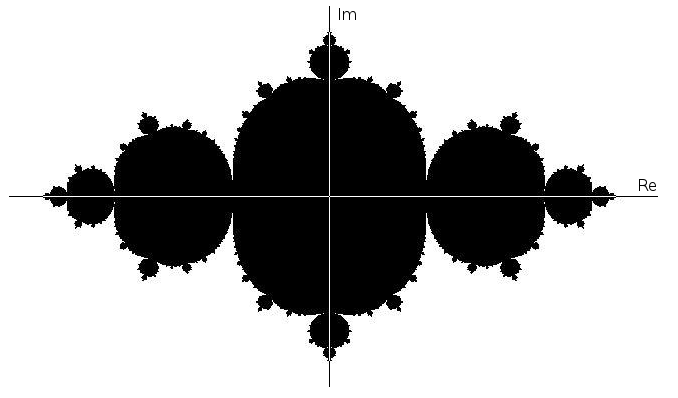
\includegraphics[width=140mm]{Figures/juliaAxes.png}
\caption{$B$ for $c = -3/4$. \textcopyright \, \href{http://www.easyfractalgenerator.com/}{easyfractalgenerator.com}}
\end{figure}
The conformal mapping theorem [cite] states that there is a holomorphic
bijection $Z$ between the open unit disc $\{z \in \Cplx\;:\;|z| < 1\}$
and the interior of $B$. Then Carath\'eodory's theorem [cite]
 states that $Z$ extends to a continuous
map from $\Circ$ to $J$. 

Let $p$ be the Hausdorff dimension of $J$ [cite]. It is known that $p \in (1,2)$ [cite].

There is a $p$-dimensional Hausdorff measure, $\Lambda_p$ on $J$ [cite].
Let
$f\in C_0(\Cplx)$ and let $\Tr_\omega$
be a Dixmier trace. We consider the quantity
\begin{equation}
    \Tr_\omega(M_{f(Z)}|\qd Z|^p).
\end{equation}


Here we see an application of our results: The results of Chapter \ref{IdealMembership}
allow us to determine which functions $\varphi$ have $\qd \varphi\in \M_{1,\infty}$,
that is, in the domain of the Dixmier trace $\Tr_\omega$.

Herein lies the utility
of quantised calculus.
It is proved by Connes in \cite[Ch. 4, Thm 17]{Connes94} that there is a non-zero constant $\lambda$,
which does not depend on $f$, such that
\begin{equation}
    \Tr_\omega(M_{f(Z)}|\qd Z|^p) = \lambda \int_J f\;d\Lambda_p.
\end{equation}
Hence the quantised calculus provides a means of computing integrals
with respect to Hausdorff measure on a Julia set.
